%%%%%%%%%%%%%%%%%%%%%%%%%%%%%%%%%%%%%%%%%%%%%%%%%%%%%%%%%%%%%%%%%%%%%%%%%%%%%%%
% Chapter 2: Desarrollo
%%%%%%%%%%%%%%%%%%%%%%%%%%%%%%%%%%%%%%%%%%%%%%%%%%%%%%%%%%%%%%%%%%%%%%%%%%%%%%%

%++++++++++++++++++++++++++++++++++++++++++++++++++++++++++++++++++++++++++++++

En el cap\'{\i}tulo anterior se ha definido el Trabajo de Fin de Grado, especificado los objetivos y actividades
a desarrollar y mencionado las tecnolog\'{\i}as empleadas para su desarrollo. A continuaci\'on, se describir\'a 
la metodolog\'{\i}a de trabajo seguida y se introducir\'a a los resultados obtenidos para posteriormente
describirlos por cap\'{\i}tulos de manera detallada.

%++++++++++++++++++++++++++++++++++++++++++++++++++++++++++++++++++++++++++++++

\section{Metodolog\'{\i}a usada}
\label{2:sec:1}

Se ha llevado a cabo una metodolog\'{\i}a de trabajo \textit{\'agil}, com\'un en el campo de la Ingenier\'{\i}a Inform\'atica,
con reuniones semanales en las que se defin\'{\i}an una serie de tareas u objetivos (iteraci\'on) y que se presentaban la siguiente semana. 
De este modo, con la entrega de prototipos funcionales de la aplicaci\'on, se han ido testeando, corrigiendo y mejorando las 
funcionalidades, al mismo tiempo que detectando problemas no contemplados en las fases previas de dise�o.

Esta metodolog\'{\i}a, adem\'as, ha propiciado la generaci\'on de ideas que se han traducido en nuevas caracter\'{\i}sticas.

%---------------------------------------------------------------------------------
\subsection{GitHub}
\label{subsec:2.1.1}

Para llevar a cabo esta metodolog\'{\i}a, se ha usado {\bfseries GitHub} como herramienta de {\bfseries Control de Versiones} (CVS).
Todo el c\'odigo implementado se alojaba en dicha herramienta, permitiendo as\'{\i} su c\'omoda modificaci\'on y actualizaci\'on.

\begin{figure}[H]
\begin{center}
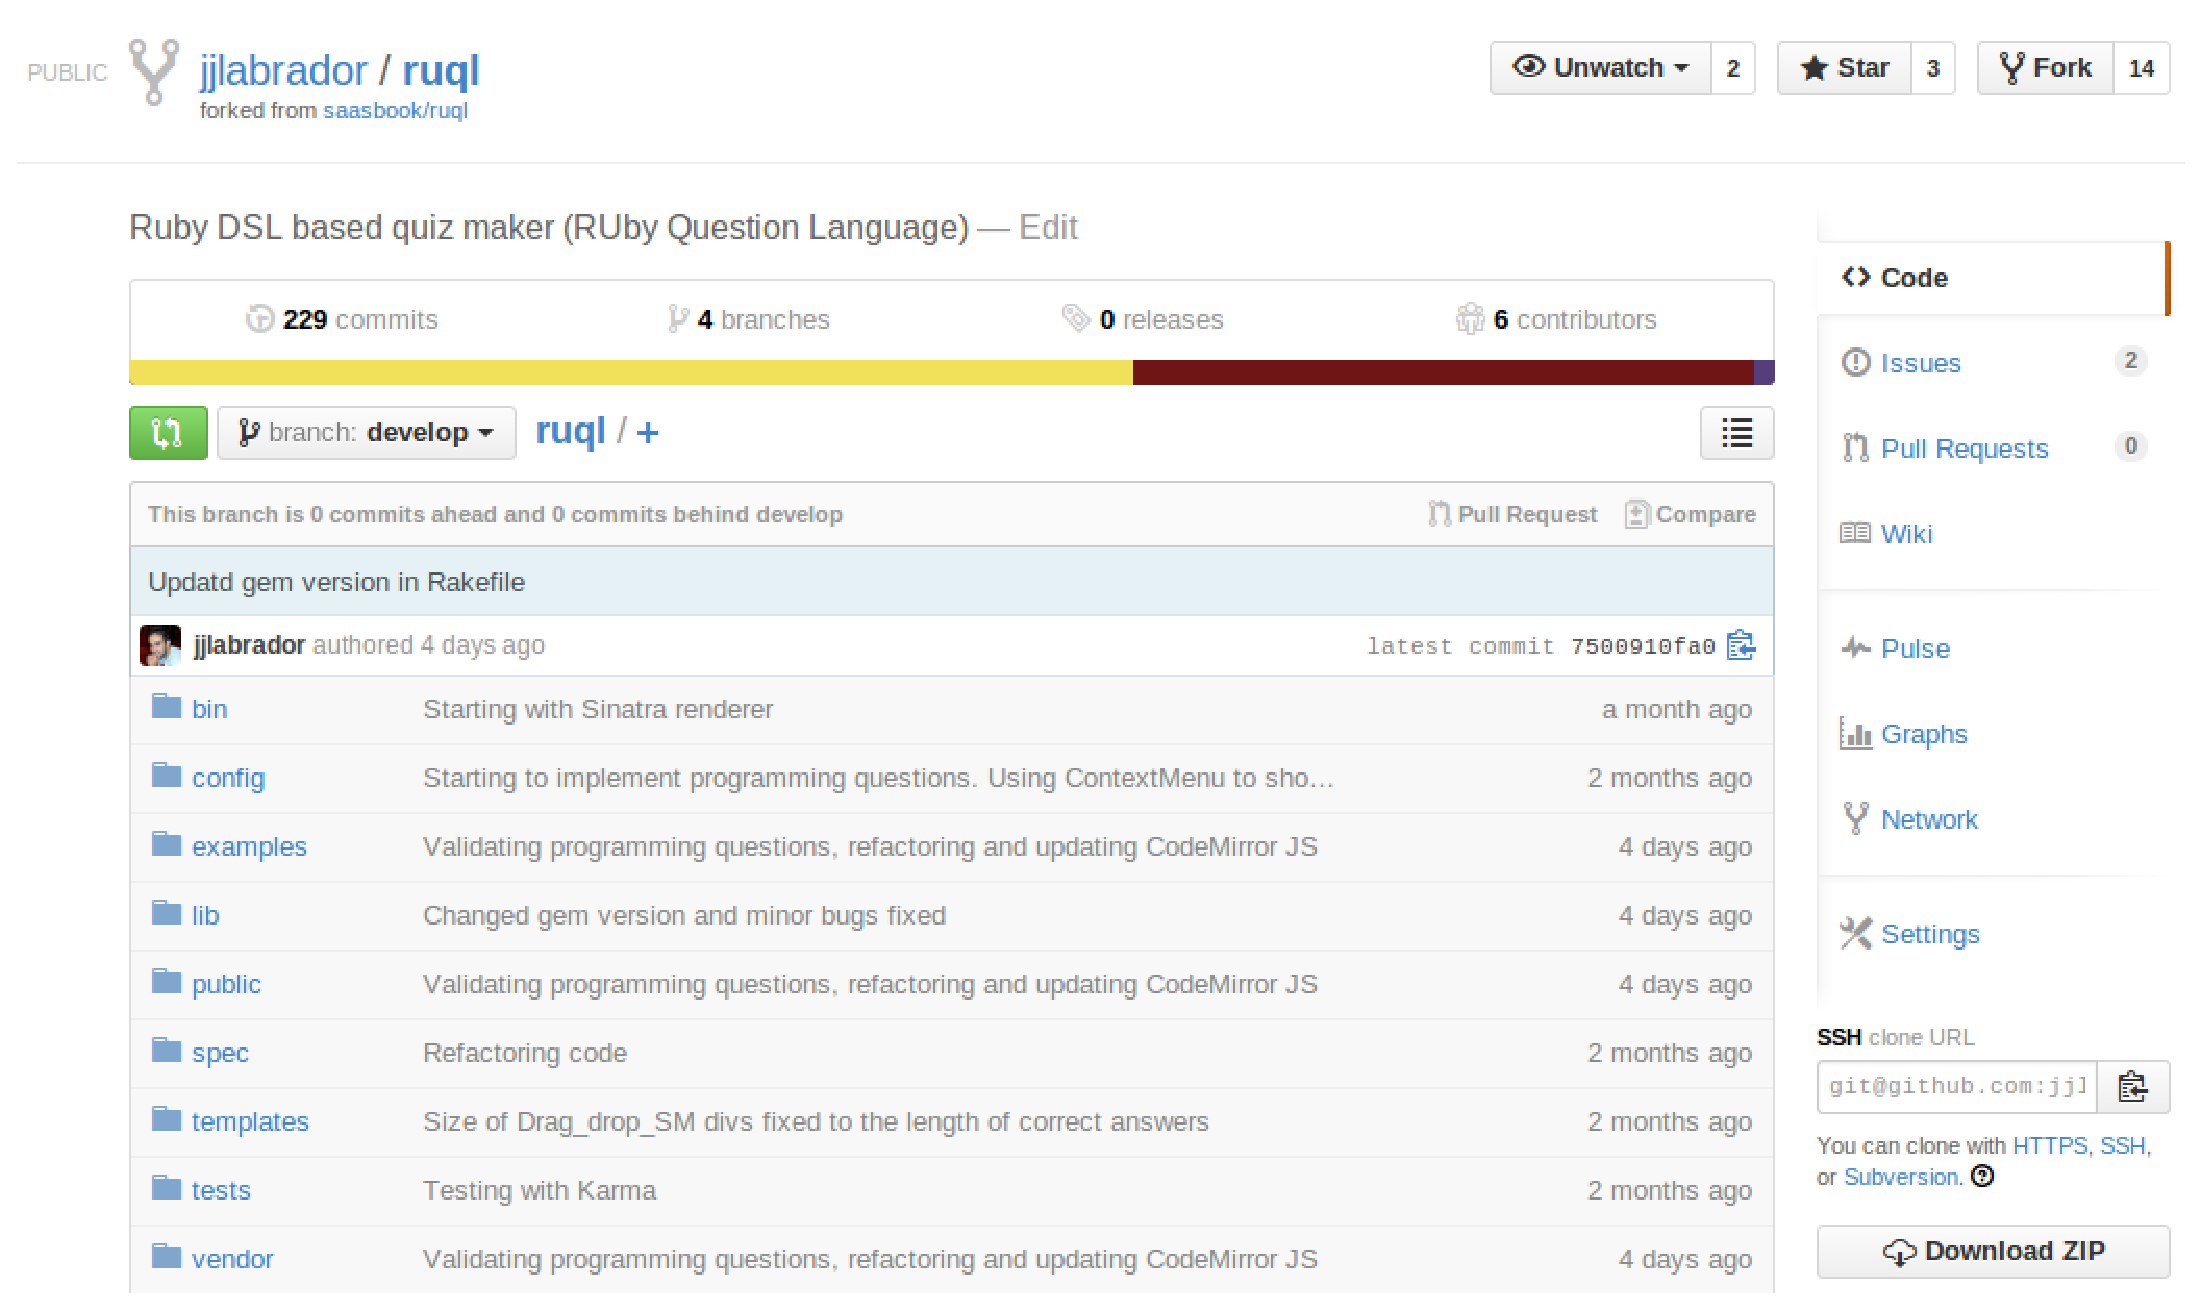
\includegraphics[width=\textwidth,height=0.58\textwidth]{images/github1.eps}
\caption{Captura del repositorio de la gema en GitHub}
\label{fig:github1}
\end{center}
\end{figure}

El trabajo se divid\'{\i}a en ramas, de modo que la versi\'on estable de la aplicaci\'on (\textit{rama master}) quedara aislada de la 
versi\'on en desarrollo (\textit{rama develop}).

\begin{figure}[H]
\begin{center}
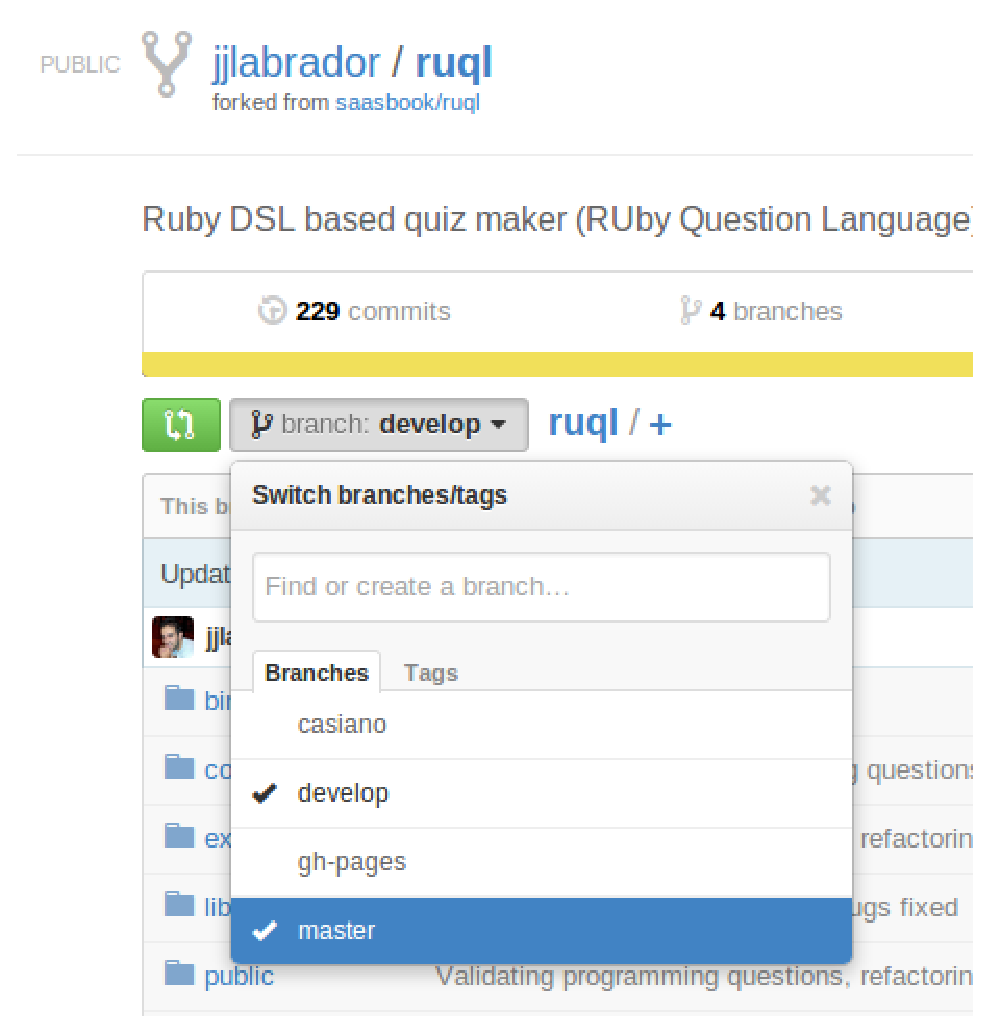
\includegraphics[width=0.47\textwidth]{images/github5.eps}
\caption{Ramas del repositorio propio}
\label{fig:github5}
\end{center}
\end{figure}

GitHub tambi\'en ha servido para mantener contacto con el creador de la gema e indicarle mi intenci\'on de mejorar su gema en mi
Trabajo de Fin de Grado. \'El ha estado al tanto de mi progreso y tras solicitarle \textit{Pull Requests} con mejoras y correcciones
de su gema me ha convertido en colaborador de su repositorio.

\begin{figure}[H]
\begin{center}

\includegraphics[width=1\textwidth]{images/github2.eps}
\caption{Pull Request aceptado y cerrado}
\label{fig:github2}
\end{center}
\end{figure}

\begin{figure}[H]
\begin{center}
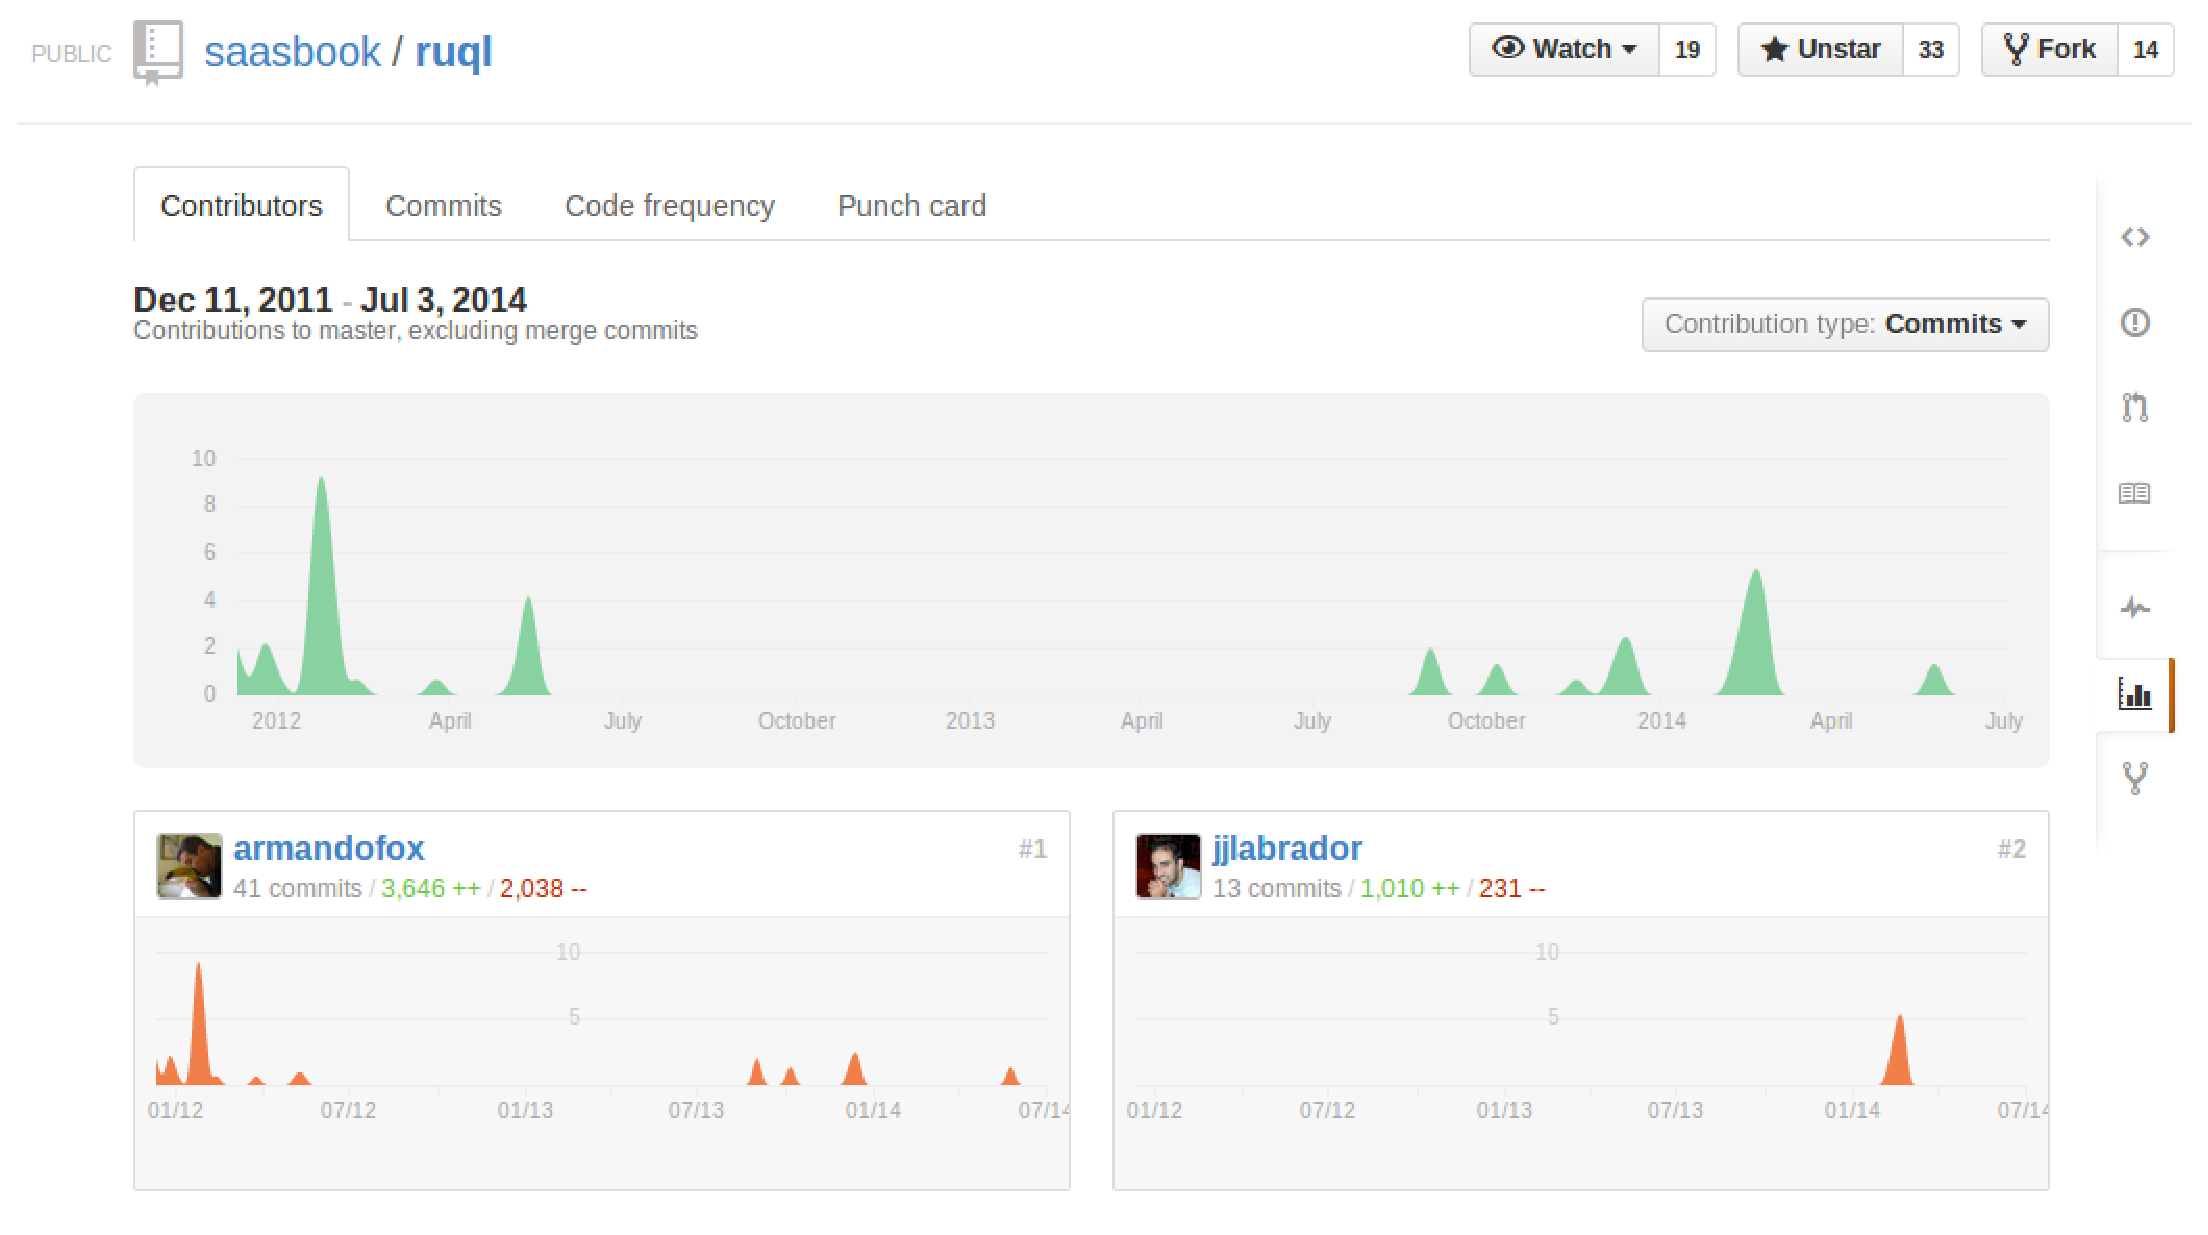
\includegraphics[width=1\textwidth]{images/github3.eps}
\caption{Contribuciones hechas al repositorio original}
\label{fig:github3}
\end{center}
\end{figure}

Las nuevas funcionalidades que han ido surgiendo, as\'{\i} como los problemas detectados, se anotaban en el apartado de \textit{issues}
con el fin de que quedara constancia de ello y se reflejara el estado en el que se encontraba cada uno.
\newpage

\begin{figure}[H]
\begin{center}
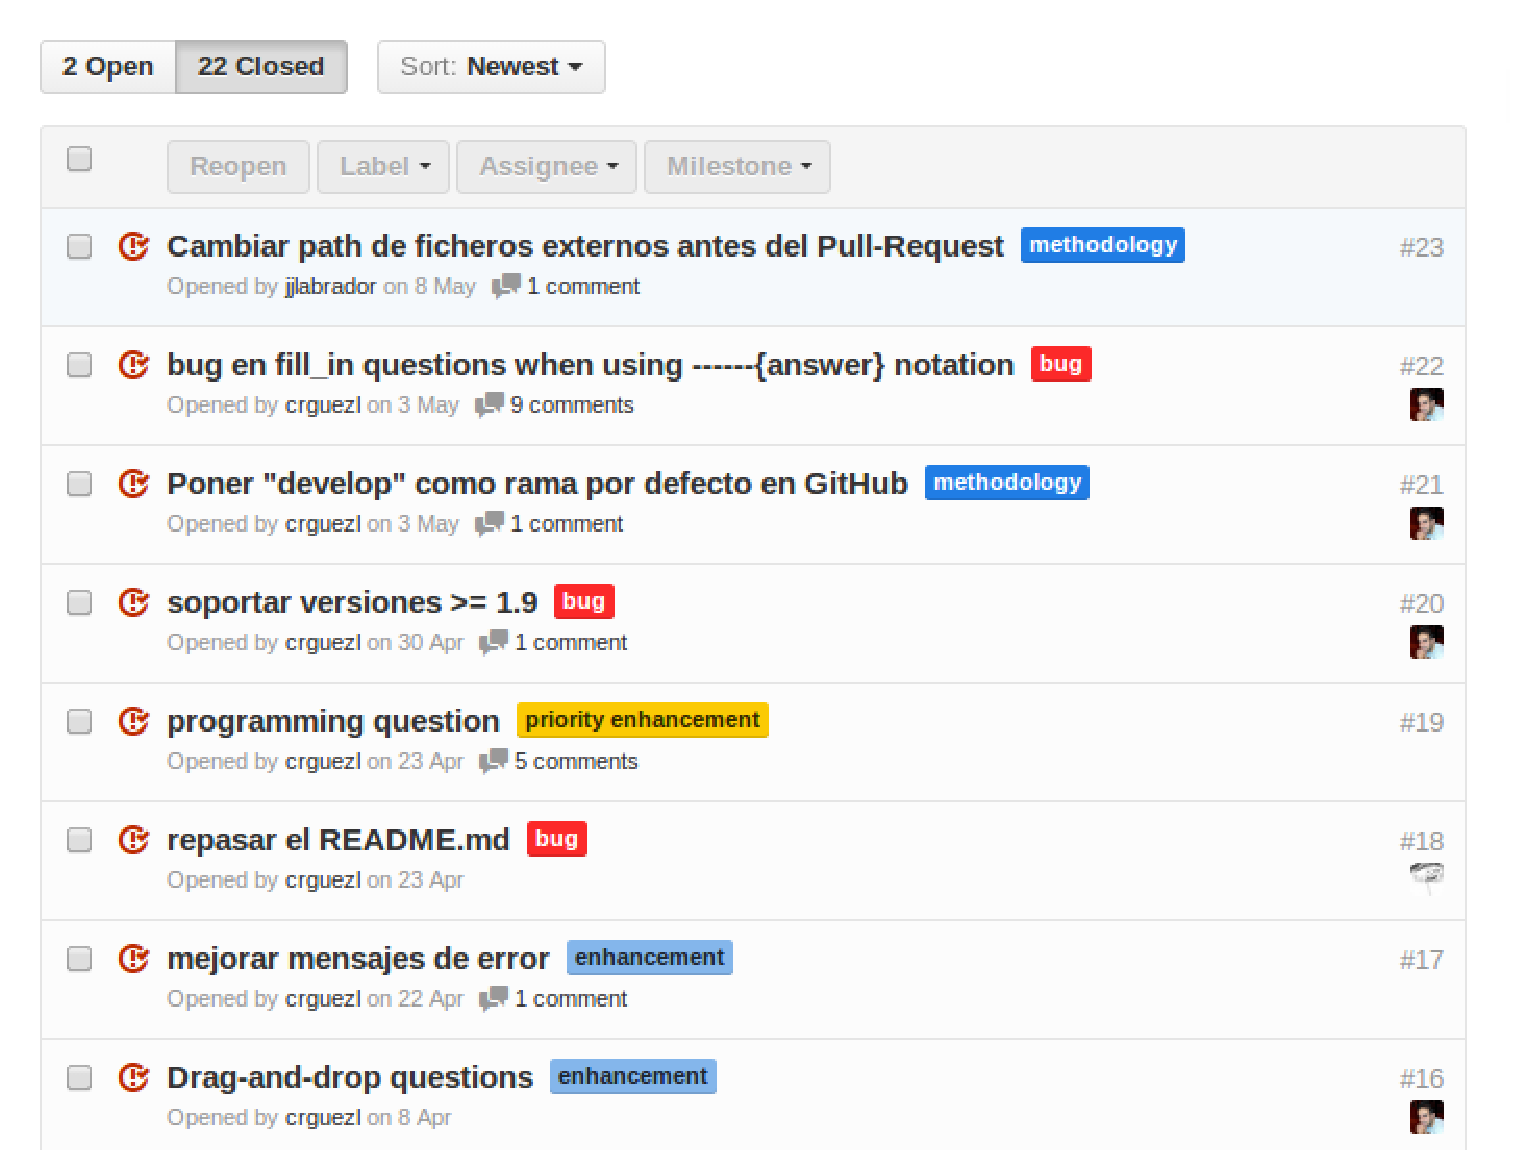
\includegraphics[width=1\textwidth]{images/github4.eps}
\caption{Apartado de issues cerrados}
\label{fig:github4}
\end{center}
\end{figure}

%---------------------------------------------------------------------------------
\subsection{Testing}
\label{subsec:2.1.2}

Dentro de la metodolog\'{\i}a tambi\'en ha habido etapas de testing, haciendo uso de la metodolog\'{\i}a de Desarrollo Dirigido por Pruebas 
{\bfseries TDD} (Test Driven Development). Se ha empleado la herramienta \textit{Spec} para los test en Ruby y se han usado los frameworks
\textit{Mocha}, \textit{Chai} y \textit{Karma} para los test del HTML y el JavaScript.

%---------------------------------------------------------------------------------
\subsection{Experiencia de usuario}
\label{subsec:2.1.3}

Por otra parte, el tutor del Trabajo de Fin de Grado ha hecho pruebas reales usando los prototipos de la aplicaci\'on con alumnos de sus asignaturas.
De este modo, se comprobaba el funcionamiento de la aplicaci\'on en un entorno real y se recibi\'a un valioso feedback para mejorar en las siguientes
iteraciones.
\bigskip

\section{Resultados}
\label{2:sec:2}

Tras el desarrollo del Trabajo de Fin de Grado, se distinguen tres claros resultados: por un lado tenemos la {\bfseries correci\'on de errores y mejoras
de la gema original}. En segunda instancia, contamos con el renderer {\bfseries HtmlForm}, v\'alido para realizar una autoevaluaci\'on propia por parte 
del alumnado que le sirve a modo de entrenamiento para afrontar el examen final. Por \'ultimo, contamos con el renderer {\bfseries Sinatra}, que genera 
una aplicaci\'on Sinatra con todo lo necesario para su despliegue y puesta en funcionamiento.

Se explicar\'an cada uno de estos resultados en los siguientes cap\'{\i}tulos de la memoria.


%---------------------------------------------------------------------------------
% \section{Problemas encontrados y soluciones}
% \label{sec:2}
% 
% A continuaci\'on se detallan los problemas encontrados durante la implementaci\'on del Trabajo de Fin de Grado y las soluciones
% encontradas para los mismos.
% 
% \subsection{Entender el funcionamiento del c\'odigo de la gema}
% \label{subsec:2.1}
% \bigskip
% 
% {\normalsize {\bfseries Soluci\'on}}
% 
% Leer la documentaci\'on de la gema, generar cuestionarios de pruebas y estudiar el c\'odigo fuente.
% 
% \subsection{Corregir tests y funcionalidades de la gema}
% \label{subsec:2.2}
% \bigskip
% 
% {\normalsize {\bfseries Soluci\'on}}
% 
% Tras realizar el correspondiente \textit{fork} en GitHub para empezar a implementar mis modificaciones, ejecut\'e los tests de la 
% gema original para comprobar la ausencia de fallos. Al finalizar, algunos tests fallaron por lo que decid\'{\i} corregirlos. Del 
% mismo modo, algunas gemas de testing existentes en el Gemfile presentaban incompatibilidades con las nuevas versiones de Ruby, por
% lo que tambi\'en se corrig\'{\i}o.
% \bigskip
% 
% Del mismo modo, las siguientes funcionalidades de la gema fueron corregidas ya que no funcionaban correctamente:
% \begin{itemize}
%   \item La opci\'on que permite indicar si el orden de las respuestas en las preguntas de completar espacios en blaco importa o no.
%   \item La opci\'on de a�adir comentarios opcionales a los textos de las preguntas.
%   \item La opci\'on \textit{raw} que permite incrustar el texto de las preguntas entre etiquetas \textless pre\textgreater \space HTML.
%   \item La opci\'on de explicaci\'on global para todos los \textit{distractors} no funcionaba.
% \end{itemize}
% 
% \subsection{Correcci\'on de preguntas de Ruby en JavaScript}
% \label{subsec:2.3}
% \bigskip
% 
% bla, bla, bla
% 
% \subsection{Correcci\'on de preguntas de JavaScript en Ruby}
% \label{subsec:2.3}
% \bigskip
% 
% bla, bla, bla
% 
% \subsection{Timeout corto entre peticiones del navegador al servidor}
% \label{subsec:2.4}
% \bigskip
% 
% bla, bla, bla
% 
% \subsection{Problema de seguridad al evaluar c\'odigo Ruby en el servidor}
% \label{subsec:2.5}
% \bigskip
% 
% bla, bla, bla
% 
% \subsection{Lugar de almacenamiento de las respuestas de los alumnos}
% \label{subsec:2.5}
% \bigskip
% 
% La idea principal era almacenar todas las preguntas y respuestas de los alumnos en una base de datos pero, viendo la evoluci\'on que ha tenido la
% herramienta Google Drive y el aumento considerable de su uso por parte de docentes, decid\'{\i} sustituir las tradicionales y siempre mon\'otonas consultas a bases de datos por esta 
% herramienta de almacenamiento que permite visualizar y administrar f\'acilmente toda la informaci\'on.